\documentclass{article}
\usepackage[utf8]{inputenc}
\usepackage{amsmath, amssymb}
\usepackage{graphicx}
\usepackage{enumitem}
\usepackage{geometry}
\usepackage{mathptmx}
\usepackage{xcolor}
\usepackage{listings}
% Code styling

\definecolor{codegreen}{rgb}{0,0.6,0}
\definecolor{codegray}{rgb}{0.5,0.5,0.5}
\definecolor{codepurple}{rgb}{0.58,0,0.82}
\definecolor{backcolour}{rgb}{0.95,0.95,0.92}

\lstset{
  language=Python,
  breaklines=true,
  breakatwhitespace=true,
  basicstyle=\ttfamily\footnotesize,
  keywordstyle=\color{codepurple},
  commentstyle=\color{codegreen},
  stringstyle=\color{red},
  captionpos=b,
  frame=single,
  showstringspaces=false,
  tabsize=4
}
\geometry{margin=1in}
\title{\textbf{Pathfinding in Rome: BFS, DFS, UCS}}
\author{Dinanath Padhya (THA078BEI010), Krishna Acharya (THA078BEI020)}
\date{}


\begin{document}
\maketitle


\section*{Introduction}
This report implements three classic search algorithms, BFS, DFS, and UCS, on a graph of 26 landmarks in Rome. We compare their paths, costs, and efficiency in solving real-world navigation tasks.

\section*{Graph Implementation}
\begin{lstlisting}[language=Python, caption={Rome City Path Finding}]
import heapq
import time
import sys
from collections import deque, defaultdict
import matplotlib.pyplot as plt
import networkx as nx
import numpy as np

class RomeCityGraph:
    def __init__(self):
        self.graph = defaultdict(list)
        self.weights = {}
        self.nodes = [
            "colosseum", "roman_forum", "palatine_hill", "capitoline_hill",
            "pantheon", "trevi_fountain", "spanish_steps", "vatican_city",
            "st_peters_basilica", "sistine_chapel", "vatican_museums",
            "castel_sant_angelo", "piazza_navona", "campo_de_fiori",
            "trastevere", "villa_borghese", "borghese_gallery", "piazza_del_popolo",
            "via_del_corso", "piazza_venezia", "circus_maximus", "baths_of_caracalla",
            "appian_way", "catacombs", "testaccio", "san_giovanni"
        ]
        
        # highway-like connections (not fully connected)
        connections = [
            ("colosseum", "roman_forum", 0.5),
            ("roman_forum", "palatine_hill", 0.2),
            ("palatine_hill", "circus_maximus", 0.5),
            ("roman_forum", "capitoline_hill", 0.4),
            ("capitoline_hill", "piazza_venezia", 0.3),
            ("piazza_venezia", "via_del_corso", 0.3),
            ("via_del_corso", "pantheon", 0.5),
            ("pantheon", "trevi_fountain", 0.8),
            ("trevi_fountain", "spanish_steps", 0.6),
            ("spanish_steps", "piazza_del_popolo", 0.7),
            ("piazza_del_popolo", "villa_borghese", 0.5),
            ("villa_borghese", "borghese_gallery", 0.2),
            ("pantheon", "piazza_navona", 0.4),
            ("piazza_navona", "campo_de_fiori", 0.4),
            ("campo_de_fiori", "trastevere", 0.8),
            ("trastevere", "vatican_city", 1.5),
            ("vatican_city", "st_peters_basilica", 0.1),
            ("vatican_city", "vatican_museums", 0.3),
            ("vatican_museums", "sistine_chapel", 0.1),
            ("st_peters_basilica", "castel_sant_angelo", 0.5),
            ("castel_sant_angelo", "piazza_navona", 1.0),
            ("trastevere", "testaccio", 1.2),
            ("testaccio", "baths_of_caracalla", 0.9),
            ("baths_of_caracalla", "circus_maximus", 0.6),
            ("circus_maximus", "colosseum", 0.8),
            ("baths_of_caracalla", "appian_way", 1.5),
            ("appian_way", "catacombs", 2.0),
            ("catacombs", "san_giovanni", 1.8),
            ("san_giovanni", "colosseum", 1.0),
            ("via_del_corso", "spanish_steps", 0.4),
            ("campo_de_fiori", "piazza_venezia", 0.7)
        ]
        
        for node1, node2, weight in connections:
            self.graph[node1].append(node2)
            self.graph[node2].append(node1)
            self.weights[(node1, node2)] = weight
            self.weights[(node2, node1)] = weight
    
    def get_neighbors(self, node):
        return self.graph[node]
    
    def get_weight(self, node1, node2):
        return self.weights.get((node1, node2), float('inf'))
    
    def visualize_graph(self):
        G = nx.Graph()
        
        for node in self.nodes:
            G.add_node(node)
        
        for (node1, node2), weight in self.weights.items():
            if not G.has_edge(node1, node2):
                G.add_edge(node1, node2, weight=weight)
        
        plt.figure(figsize=(14, 10))
        pos = nx.spring_layout(G, k=2, iterations=100, seed=42)
        
        nx.draw_networkx_nodes(G, pos, node_color='lightblue', 
                              node_size=1000, alpha=0.9)
        nx.draw_networkx_labels(G, pos, font_size=7, font_weight='bold')
        nx.draw_networkx_edges(G, pos, alpha=0.7, width=2)
        
        edge_labels = nx.get_edge_attributes(G, 'weight')
        nx.draw_networkx_edge_labels(G, pos, edge_labels, font_size=6)
        
        plt.title("rome city graph - landmarks and connections", fontsize=14)
        plt.axis('off')
        plt.tight_layout()
        plt.show()

class GraphSearchAlgorithms:
    def __init__(self, graph):
        self.graph = graph
        self.complexity_data = {}
    
    def measure_complexity(self, algorithm_name, func, *args, **kwargs):
        start_time = time.perf_counter()
        result = func(*args, **kwargs)
        end_time = time.perf_counter()
        execution_time = end_time - start_time
        
        path, visited_order, max_memory = result
        
        self.complexity_data[algorithm_name] = {
            'time': execution_time,
            'space': max_memory,
            'nodes_visited': len(visited_order),
            'path_length': len(path) if path else 0,
            'path': path,
            'visited_order': visited_order
        }
        
        return result
    
    def bfs(self, start, goal):
        if start not in self.graph.nodes or goal not in self.graph.nodes:
            return [], [], 0
        
        queue = deque([(start, [start])])
        visited = set()
        visited_order = []
        max_memory = 0
        
        while queue:
            current_memory = sys.getsizeof(queue) + sys.getsizeof(visited)
            max_memory = max(max_memory, current_memory)
            
            current, path = queue.popleft()
            
            if current in visited:
                continue
                
            visited.add(current)
            visited_order.append(current)
            
            if current == goal:
                return path, visited_order, max_memory
            
            neighbors = self.graph.get_neighbors(current)
            for neighbor in neighbors:
                if neighbor not in visited:
                    new_path = path + [neighbor]
                    queue.append((neighbor, new_path))
        
        return [], visited_order, max_memory
    
    def dfs(self, start, goal):
        if start not in self.graph.nodes or goal not in self.graph.nodes:
            return [], [], 0
        
        stack = [(start, [start])]
        visited = set()
        visited_order = []
        max_memory = 0
        
        while stack:
            current_memory = sys.getsizeof(stack) + sys.getsizeof(visited)
            max_memory = max(max_memory, current_memory)
            
            current, path = stack.pop()
            
            if current in visited:
                continue
                
            visited.add(current)
            visited_order.append(current)
            
            if current == goal:
                return path, visited_order, max_memory
            
            neighbors = self.graph.get_neighbors(current)
            for neighbor in reversed(neighbors):
                if neighbor not in visited:
                    new_path = path + [neighbor]
                    stack.append((neighbor, new_path))
        
        return [], visited_order, max_memory
    
    def ucs(self, start, goal):
        if start not in self.graph.nodes or goal not in self.graph.nodes:
            return [], [], 0
        
        pq = [(0, start, [start])]
        visited = set()
        visited_order = []
        max_memory = 0
        
        while pq:
            current_memory = sys.getsizeof(pq) + sys.getsizeof(visited)
            max_memory = max(max_memory, current_memory)
            
            cost, current, path = heapq.heappop(pq)
            
            if current in visited:
                continue
                
            visited.add(current)
            visited_order.append(current)
            
            if current == goal:
                return path, visited_order, max_memory
            
            neighbors = self.graph.get_neighbors(current)
            for neighbor in neighbors:
                if neighbor not in visited:
                    edge_cost = self.graph.get_weight(current, neighbor)
                    new_cost = cost + edge_cost
                    new_path = path + [neighbor]
                    heapq.heappush(pq, (new_cost, neighbor, new_path))
        
        return [], visited_order, max_memory
    
    def compare_algorithms(self, start, goal):
        print(f"searching from {start} to {goal}")
        print("-" * 50)
        
        algorithms = [("bfs", self.bfs), ("dfs", self.dfs), ("ucs", self.ucs)]
        
        for name, algorithm in algorithms:
            self.measure_complexity(name, algorithm, start, goal)
        
        self.print_results()
        self.visualize_comparison()
    
    def print_results(self):
        print("\nresults:")
        print("-" * 80)
        
        for alg_name, data in self.complexity_data.items():
            print(f"\n{alg_name}:")
            if data['path']:
                print(f"  shortest path: {' -> '.join(data['path'])}")
                
                # calculate total distance
                total_distance = 0
                for i in range(len(data['path']) - 1):
                    total_distance += self.graph.get_weight(data['path'][i], data['path'][i+1])
                print(f"  total distance: {total_distance:.1f} km")
            else:
                print("  no path found")
            
            print(f"  visited order: {' -> '.join(data['visited_order'])}")
            print(f"  nodes visited: {data['nodes_visited']}")
            print(f"  time taken: {data['time']*1000:.4f} ms")
            print(f"  space used: {data['space']} bytes")
        
        print("\ncomplexity analysis:")
        print("-" * 50)
        print("algorithm | time (ms) | space (bytes) | nodes visited | path length")
        print("-" * 70)
        
        for alg_name, data in self.complexity_data.items():
            print(f"{alg_name:<9} | {data['time']*1000:<9.4f} | {data['space']:<13} | "
                  f"{data['nodes_visited']:<13} | {data['path_length']}")
    
    def visualize_comparison(self):
        if not self.complexity_data:
            return
        
        algorithms = list(self.complexity_data.keys())
        times = [self.complexity_data[alg]['time'] * 1000 for alg in algorithms]
        spaces = [self.complexity_data[alg]['space'] for alg in algorithms]
        nodes_visited = [self.complexity_data[alg]['nodes_visited'] for alg in algorithms]
        path_lengths = [self.complexity_data[alg]['path_length'] for alg in algorithms]
        
        fig, ((ax1, ax2), (ax3, ax4)) = plt.subplots(2, 2, figsize=(12, 8))
        
        colors = ['#ff6b6b', '#4ecdc4', '#45b7d1']
        
        # time comparison
        bars1 = ax1.bar(algorithms, times, color=colors)
        ax1.set_title('execution time')
        ax1.set_ylabel('time (ms)')
        for i, bar in enumerate(bars1):
            height = bar.get_height()
            ax1.text(bar.get_x() + bar.get_width()/2., height,
                    f'{height:.4f}', ha='center', va='bottom', fontsize=8)
        
        # space comparison
        bars2 = ax2.bar(algorithms, spaces, color=colors)
        ax2.set_title('memory usage')
        ax2.set_ylabel('memory (bytes)')
        for i, bar in enumerate(bars2):
            height = bar.get_height()
            ax2.text(bar.get_x() + bar.get_width()/2., height,
                    f'{int(height)}', ha='center', va='bottom', fontsize=8)
        
        # nodes visited
        bars3 = ax3.bar(algorithms, nodes_visited, color=colors)
        ax3.set_title('nodes visited')
        ax3.set_ylabel('number of nodes')
        for i, bar in enumerate(bars3):
            height = bar.get_height()
            ax3.text(bar.get_x() + bar.get_width()/2., height,
                    f'{int(height)}', ha='center', va='bottom', fontsize=8)
        
        # path length
        bars4 = ax4.bar(algorithms, path_lengths, color=colors)
        ax4.set_title('path length')
        ax4.set_ylabel('path length (nodes)')
        for i, bar in enumerate(bars4):
            height = bar.get_height()
            ax4.text(bar.get_x() + bar.get_width()/2., height,
                    f'{int(height)}', ha='center', va='bottom', fontsize=8)
        
        plt.suptitle('algorithm performance comparison', fontsize=14)
        plt.tight_layout()
        plt.show()

def main():
    rome_graph = RomeCityGraph()
    
    print("rome city graph search algorithms")
    print(f"graph created with {len(rome_graph.nodes)} landmarks")
    
    rome_graph.visualize_graph()
    
    search_algorithms = GraphSearchAlgorithms(rome_graph)
    
    # main comparison
    start_node = "colosseum"
    goal_node = "vatican_city"
    search_algorithms.compare_algorithms(start_node, goal_node)


\end{lstlisting}
\section*{Discussion and Results}

\noindent
\textbf{Test Case:} \textit{Colosseum → Vatican City}

\vspace{0.3cm}
\begin{itemize}
    \item \textbf{BFS:}
          Path:
          \texttt{colosseum → circus\_maximus → baths\_of\_caracalla → testaccio → trastevere → vatican\_city}
          Total distance: \textbf{5.0 km}
          Nodes visited: \textbf{18}
          Time: \textbf{0.1634 ms}
          Memory used: \textbf{1488 bytes}

    \item \textbf{DFS:}
          Path:
          \texttt{colosseum → roman\_forum → palatine\_hill → circus\_maximus → baths\_of\_caracalla → testaccio → trastevere → campo\_de\_fiori → piazza\_navona → castel\_sant\_angelo → st\_peters\_basilica → vatican\_city}
          Total distance: \textbf{6.7 km}
          Nodes visited: \textbf{21}
          Time: \textbf{0.1354 ms}
          Memory used: \textbf{2416 bytes}

    \item \textbf{UCS:}
          Path:
          \texttt{colosseum → roman\_forum → capitoline\_hill → piazza\_venezia → campo\_de\_fiori → piazza\_navona → castel\_sant\_angelo → st\_peters\_basilica → vatican\_city}
          Total distance: \textbf{3.9 km}
          Nodes visited: \textbf{24}
          Time: \textbf{0.2756 ms}
          Memory used: \textbf{2384 bytes}
\end{itemize}

\vspace{0.4cm}
\noindent
\textbf{Complexity Summary Table}:

\begin{center}
    \begin{tabular}{|l|c|c|c|c|}
        \hline
        \textbf{Algorithm} & \textbf{Time (ms)} & \textbf{Memory (bytes)} & \textbf{Nodes Visited} & \textbf{Path Length} \\
        \hline
        BFS                & 0.1634             & 1488                    & 18                     & 6                    \\
        DFS                & 0.1354             & 2416                    & 21                     & 12                   \\
        UCS                & 0.2756             & 2384                    & 24                     & 9                    \\
        \hline
    \end{tabular}
\end{center}

\vspace{0.6cm}
\begin{figure}[!h]
    \centering
    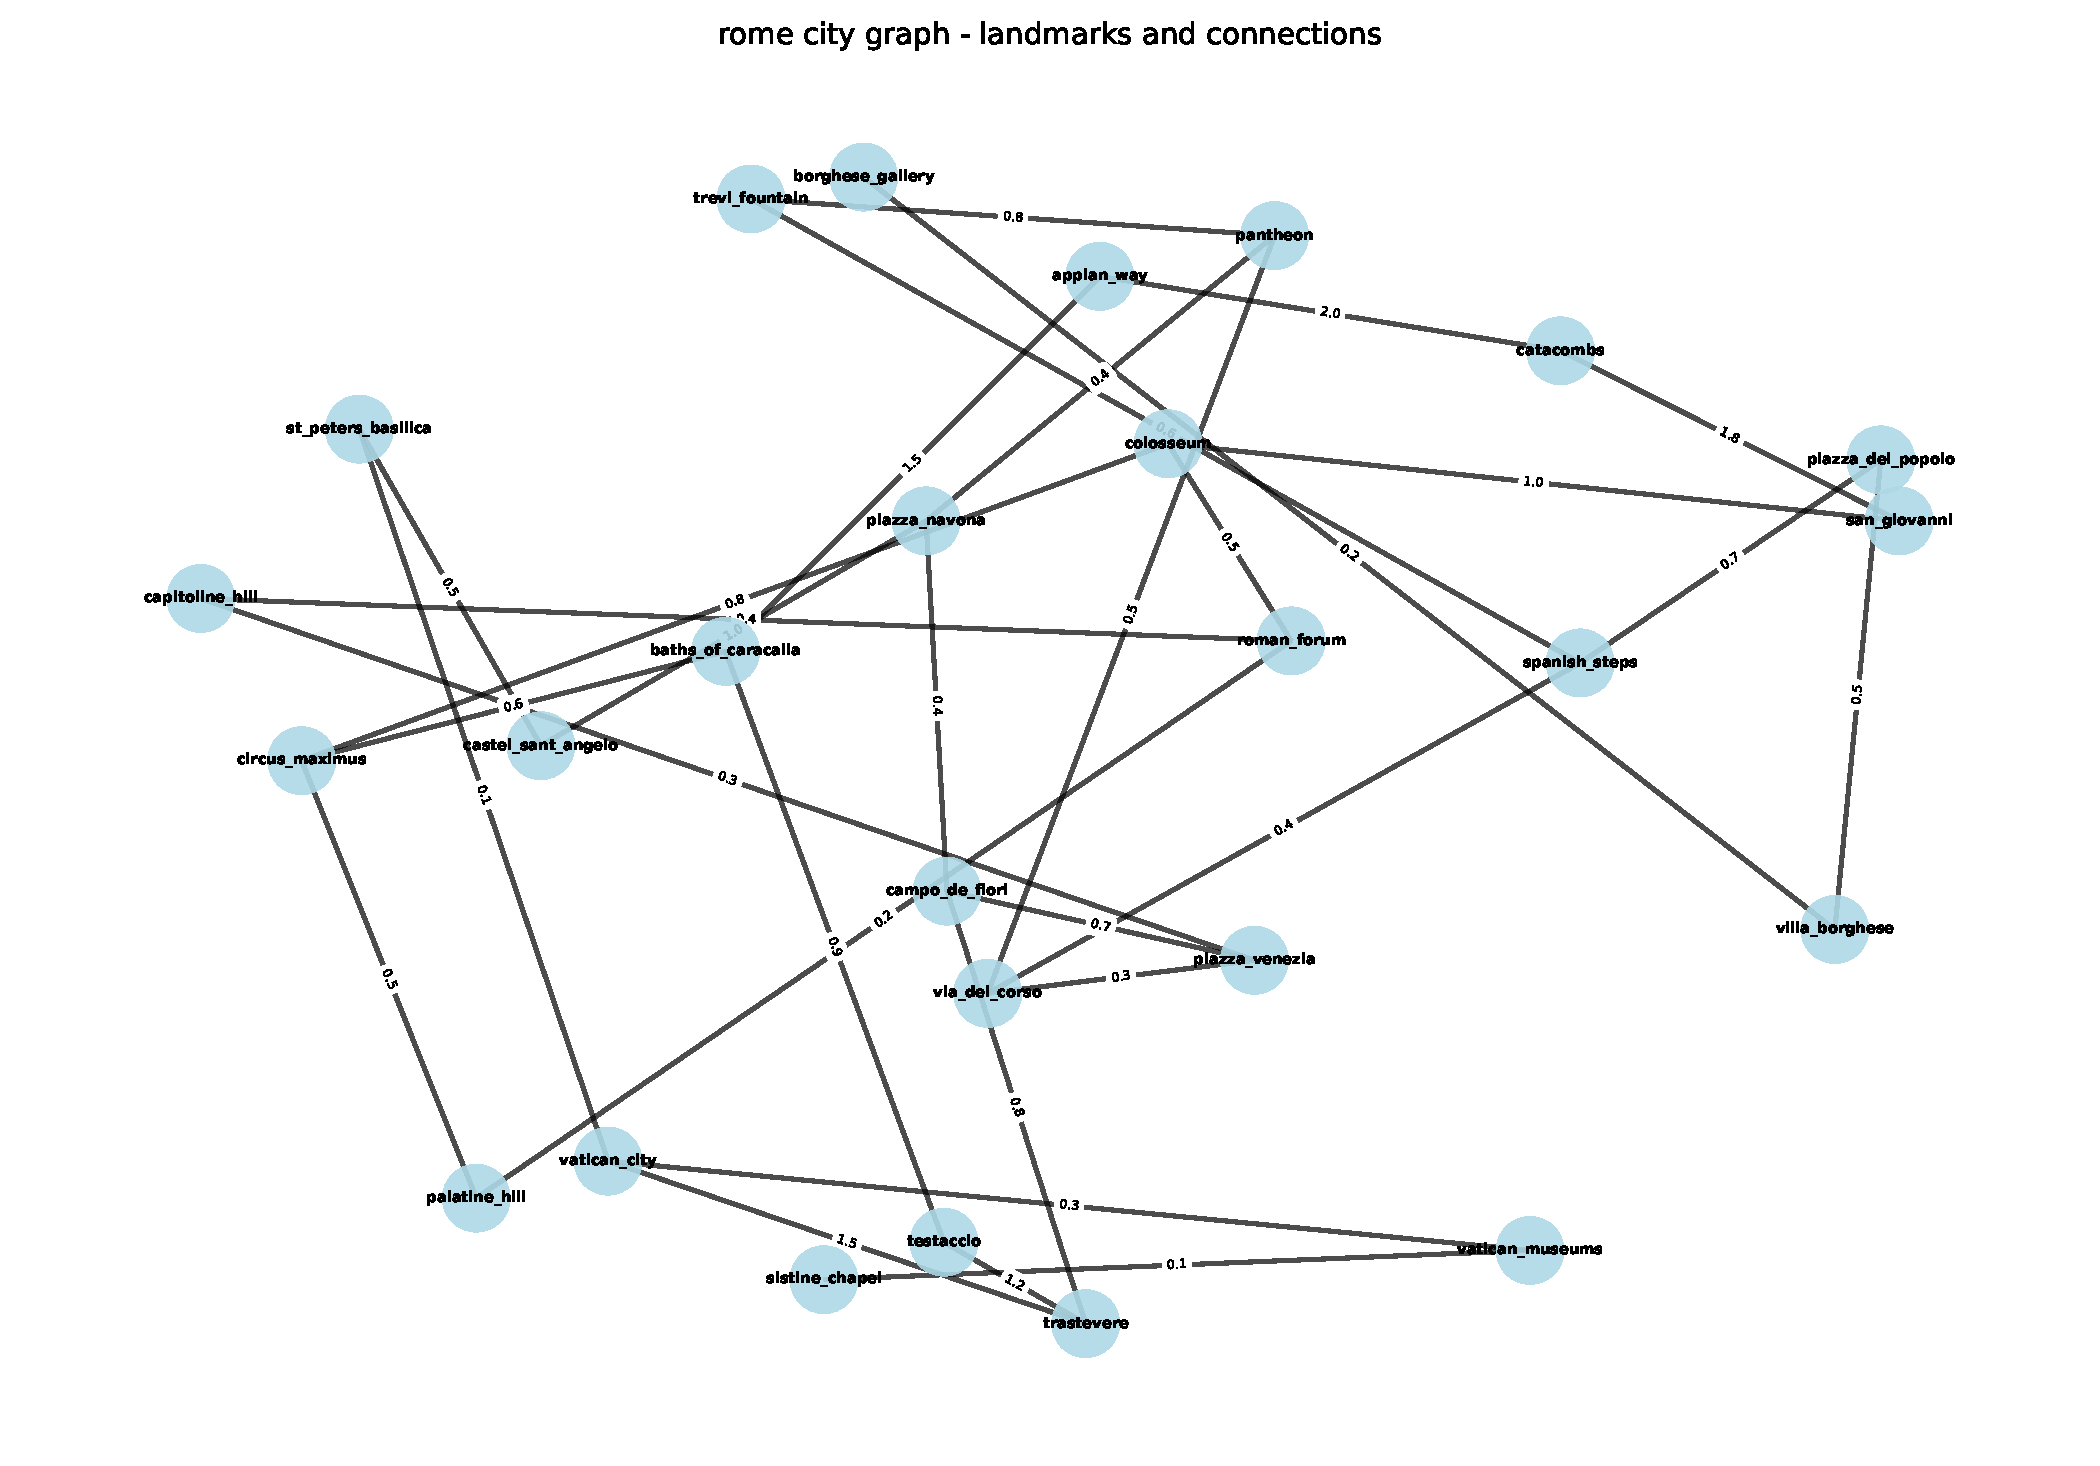
\includegraphics[width=0.85\textwidth]{./figs/graph.pdf}
    \caption{Rome City Graph with 26 Landmarks and Connections}
\end{figure}

\begin{figure}[!h]
    \centering
    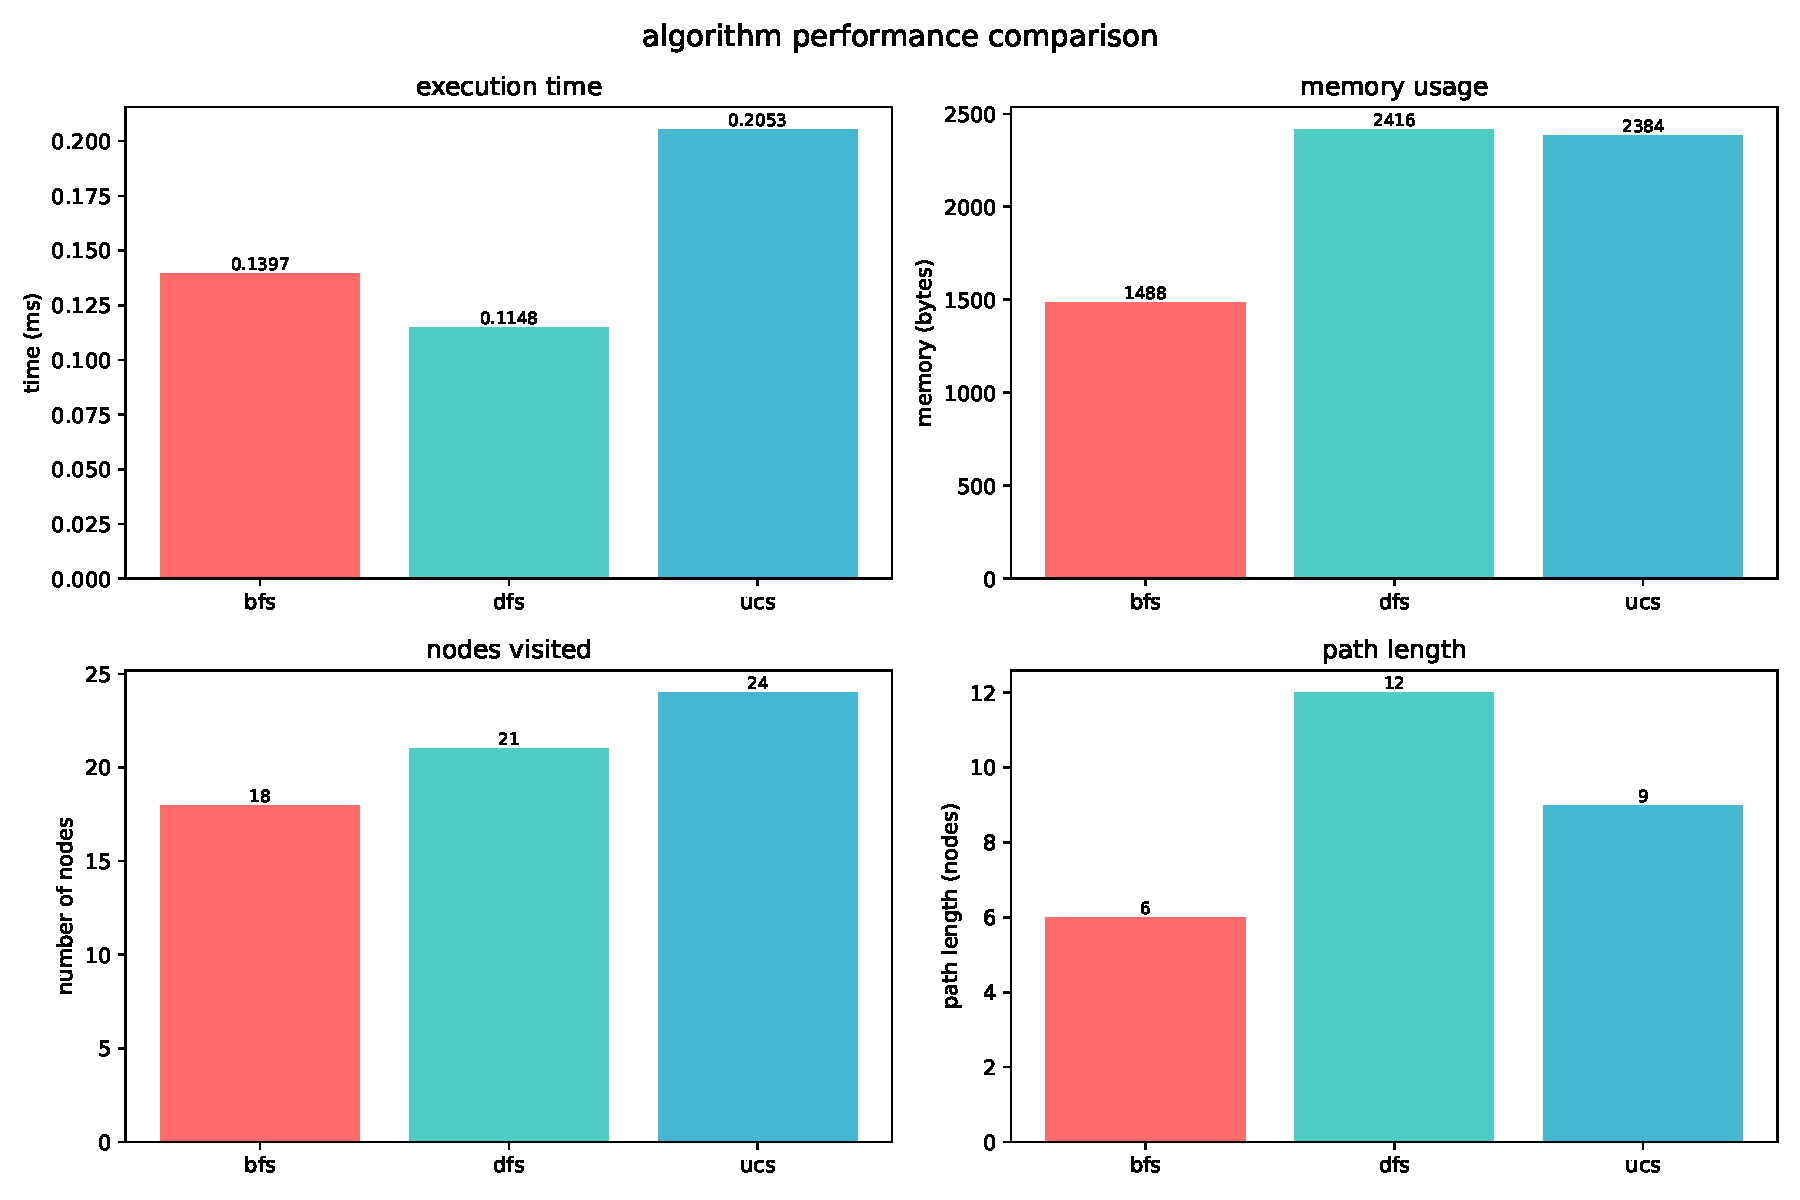
\includegraphics[width=0.85\textwidth]{./figs/algo.pdf}
    \caption{Performance Comparison of BFS, DFS, and UCS}
\end{figure}

\section*{Conclusion}

The choice of algorithm depends on the problem’s goals:

\begin{itemize}
    \item \textbf{BFS} offers a good balance between performance and correctness, finding a fairly short path efficiently in both time and memory.
    \item \textbf{DFS} explores paths quickly and uses slightly more memory, but can end up with longer and non-optimal paths due to its deep traversal.
    \item \textbf{UCS} guarantees the shortest distance path, making it ideal for applications where cost optimization is critical, though at the cost of more time and space.
\end{itemize}

In this scenario, UCS performed best in terms of distance, BFS was fastest for a reasonably good route, and DFS, while quickest, resulted in the longest travel distance.

\end{document}